\documentclass{scrartcl}
\usepackage{hyperref}
\usepackage{tikz}
\usetikzlibrary{patterns}
\usepackage{subcaption}
\usepackage{pifont}
\usepackage{graphicx}
\newcommand{\vampire}{{Vampire}}
\newcommand{\iprover}{iProver}
\newcommand{\E}{{\textsc E}}
\newcommand{\zthree}{{\textsc Z3}}
\newcommand{\tick}{\ding{51}}
\newcommand{\cross}{\ding{55}}

\title{Dynamic Strategy Priority: \\ Empower the strong and abandon the weak\footnote{Originally an extended abstract by the same authors that will be presented at AITP, March 2018. Re-purposed for COMP80142.}.}
\author{
 Michael Rawson \and 
 Giles Reger
}

\begin{document}
\maketitle
\begin{abstract}
\noindent
A key usability factor in interactive theorem proving is the time taken for automation tools to complete.
Automated theorem provers run lists of proof strategies sequentially, which can cause proofs to be found more slowly than necessary.
We show that it is possible to predict which strategies are likely to succeed while they are running using an artificial neural network.
We also implement a run-time strategy scheduler in the \vampire{} prover which improves average proof search time, and hence increases usability for interactive theorem proving.
\end{abstract}

\section{Introduction}
Modern automated theorem provers (e.g. \E{}~\cite{E}, \iprover{}~\cite{iProver}, \vampire{}~\cite{Vampire}, CVC4 \cite{CVC4}) for first-order logic rely on \emph{portfolio modes}~\cite{portfolio}, which utilise hundreds of distinct \emph{strategies}.
Of these strategies, only a few might solve a hard problem, often rapidly.
Typically, a portfolio of strategies has a pre-defined execution order: the prover will process strategies in this order, running each until a winning strategy is found or the prover runs out of time.

Portfolio modes are important as, in practice, there is no best strategy.
Furthermore, it is uncommon that two hard problems are efficiently solved by the same strategy.
However, portfolio execution is not without problems: deciding the optimal ordering and time allocation is hard in general~\cite{predict-success}, and produces overly-rigid, brittle engineering when applied to specific domains, such as those found in the TPTP problem set~\cite{TPTP}.
Moreover, for any particular problem, some lengthy strategies that are successful on other problems are doomed to failure from the outset --- see Figure \ref{fig:blocking} --- but are left to run unchecked by the prover, wasting time that could be spent on more productive strategies.

\begin{figure}
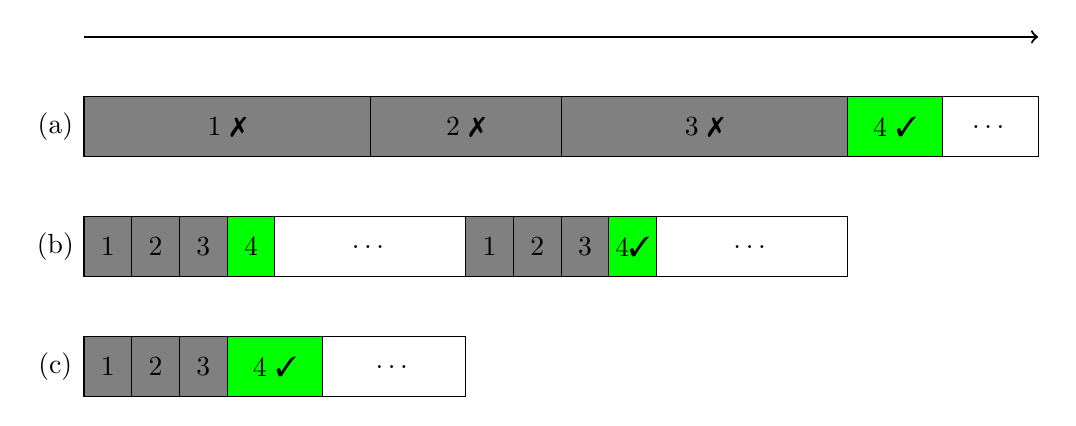
\begin{tikzpicture}[x=0.01\textwidth, y=.3in]
	\draw[thick, ->] (0, 6) -- (100, 6) node {};

	\draw (-3, 4.5) node {(a)};
	\draw[fill=gray] (0, 4) rectangle (30, 5) node [midway] {1 \cross};
	\draw[fill=gray] (30, 4) rectangle (50, 5) node [midway] {2 \cross};
	\draw[fill=gray] (50, 4) rectangle (80, 5) node [midway] {3 \cross};
	\draw[fill=green] (80, 4) rectangle (90, 5) node [midway] {4 \tick};
	\draw (90, 4) rectangle (100, 5) node [midway] {\ldots};

	\draw (-3, 2.5) node {(b)};
	\draw[fill=gray] (0, 2) rectangle (5, 3) node [midway] {1};
	\draw[fill=gray] (5, 2) rectangle (10, 3) node [midway] {2};
	\draw[fill=gray] (10, 2) rectangle (15, 3) node [midway] {3};
	\draw[fill=green] (15, 2) rectangle (20, 3) node [midway] {4};
	\draw (20, 2) rectangle (40, 3) node [midway] {\ldots};
	\draw[fill=gray] (40, 2) rectangle (45, 3) node [midway] {1};
	\draw[fill=gray] (45, 2) rectangle (50, 3) node [midway] {2};
	\draw[fill=gray] (50, 2) rectangle (55, 3) node [midway] {3};
	\draw[fill=green] (55, 2) rectangle (60, 3) node [midway] {4\tick};
	\draw (60, 2) rectangle (80, 3) node [midway] {\ldots};

	\draw (-3, 0.5) node {(c)};
	\draw[fill=gray] (0, 0) rectangle (5, 1) node [midway] {1};
	\draw[fill=gray] (5, 0) rectangle (10, 1) node [midway] {2};
	\draw[fill=gray] (10, 0) rectangle (15, 1) node [midway] {3};
	\draw[fill=green] (15, 0) rectangle (25, 1) node [midway] {4 \tick};
	\draw (25, 0) rectangle (40, 1) node [midway] {\ldots};
\end{tikzpicture}
\caption{Several strategy schedules and their effects. (a) Failing strategies might block a successful strategy. (b) Round-robin scheduling can help mitigate this problem. (c) This approach is improved if promising strategies run for longer.}
\label{fig:blocking}
\end{figure}

In this work we first demonstrate correlation between trends in dynamic properties of proof search, and the pending success or failure of a strategy.
We then utilise this to implement strategy scheduling, prioritising those strategies most likely to succeed.
This approach differs from previous work~\cite{E,static1,static2} which attempts to predict successful strategies \emph{a priori} from static features of the input problem; instead we tip running strategies for success based on dynamic, run-time features and use this information to make decisions at runtime. 

\section{Data collection and processing}
In order to identify a correlation, some data is required.
Modifying Vampire to log execution data (such as memory usage, or more specific metrics such as the number of generated clauses) for different strategies obtained from its primary portfolio mode\footnote{CASC-mode, a portfolio designed for the CASC competition~\cite{CASC}.} is straightforward, but some data-collection decisions were made:
\begin{itemize}
	\item Only numerical data immediately available in the prover was collected, but there is scope here for both non-numeric and derivative data sources, which may provide greater insight into the proof state in future work.
	\item Data was collected at intervals of a fixed number of internal resolution steps. This may not necessarily correspond to fixed time intervals, as each step may be more or less expensive, depending on the strategy and the problem.
	\item All available data was collected, even if it emerged to be constant or unhelpful. This allowed an agnostic approach to learning in which the neural network training procedure selected relevant features.
\end{itemize}
In all, 376 features are recorded.
The execution traces produced are difficult to work with, however: some are short or non-existent, others are extremely lengthy.
Some feature values also have an extremely high variance.
To deal with these problems, a post-processing step is applied.
For each feature, the mean over the entire data set is then mapped to 0, and the dataset is scaled to unit variance.
Data that are too short are discarded (the strategy likely did not take very long in any case), and then a time average is taken over 10 ``buckets'' to produce a fixed trace size.
An example post-processed trace is shown in figure \ref{fig:trace}.

\begin{figure}
	\includegraphics[width=\textwidth]{plot}
	\caption{An example trace, displayed as a colourmap, after post-processing.}
	\label{fig:trace}
\end{figure}

\section{Predicting successful strategies}
Being able to predict which traces are going to succeed in time, and which will fail at first seems unlikely.
However, it is known that the ``slowly-growing search space'' maxim, which states that strategies which minimise the number of derived clauses over time are more likely to succeed, is an effective heuristic for finding good strategies in saturation-based theorem proving~\cite{predict-success}.
Since the data we use includes the number of derived clauses, among many other features, it appears more plausible that this approach might work at least as well as the slow-growth heuristic alone.
Engineering a prediction algorithm that attempts to partition traces into ``succeeding'' and ``failing'' classes is possible with the use of modern machine-learning techniques.
Conveniently, these methods do not usually produce a binary output, but instead some \(f(\mathbf{X}) \in \left[0, 1\right]\) which might be seen as the ``level of confidence'' in success of the trace, \(\mathbf{X}\).
This success score can be used to apply an ordering to executing strategies, allowing ``smart'' dynamic scheduling of strategies.

In particular, we evaluated:
\begin{enumerate}
	\item A simple neural network with one input for each datum in the trace and a single hidden layer.
	\item A convolutional network~\cite{cnn} which performed a 1-dimensional convolutional pass along the time axis for each feature before the hidden layer.
	\item A recurrent network~\cite{gru}, feeding the time series into a gated recurrent unit before processing.
\end{enumerate}
Results for this classification task are shown in figure \ref{fig:xvalidation}.
Both of the more-advanced classifiers performed better than the simple neural network.
However, the simple network was chosen for integration into Vampire for implementation simplicity, and for performance reasons --- it is ``good enough''.

\begin{figure}
	\centering
	\begin{tabular}{c c c}
		Method & Mean Accuracy & Standard Deviation\\
		\hline
		Simple neural network & 81.5\% & 2.0\%\\
		Convolutional network & 82.4\% & 3.1\%\\
		Recurrent network & 83.9\% & 1.9\%\\
	\end{tabular}
	\caption{\(k\)-fold cross-validation classification accuracy on a balanced dataset of succeeding and failing execution traces. \(k=5\).}
	\label{fig:xvalidation}
\end{figure}

\section{Intelligent scheduling for Vampire}
We show that this abstract predictor can be used in a concrete implementation for the Vampire prover.
In the modified prover, it is used to run several strategies from Vampire's portfolio in a modified scheduler: strategies self-report their own execution data to the supervisor process and halt for re-evaluation at regular intervals.
When a strategy halts, the scheduler then decides whether to re-schedule the strategy for some more time, or to swap it out for a different strategy.
The algorithm used is as follows, taking as input a set of strategies to run:
\begin{enumerate}
	\item Initialize an empty ``run pool'' of processes, with a maximum size equal to the desired number of workers (e.g. CPU cores available). Also initialize an empty priority queue of paused processes.
	\item Whenever the pool is under capacity, take the following steps:
	\begin{enumerate}
		\item If the best process in the paused queue has a priority greater than the static priority \(p_\textrm{static}\), wake it and move it into the running pool. In tests, a static priority of around 0.5 appeared to work best.
		\item Otherwise, take a new strategy from the input set and start a new process to run that strategy.
		\item If the input set is empty, take the process from the queue regardless of its priority.
	\end{enumerate}
	\item When a strategy pauses:
	\begin{enumerate}
		\item Remove the process from the pool.
		\item Re-evaluate the process priority using the neural network and the data it provided.
		\item Insert the process into the queue with the computed priority.
	\end{enumerate}
	\item When a strategy terminates, check if it succeeded. Otherwise, remove it from the pool.
	\item If the pool, the queue, and the set of input strategies are all depleted, all strategies have failed. Exit.
\end{enumerate}

\section{Benchmark results}
The modified prover (\(M\)) was compared against a recent release of Vampire (\(V\)) under identical conditions on the TPTP benchmark, containing around 20,000 relevant problems.
The two provers performed similarly in terms of the number of problems solved.
The baseline \(V\) proved 585 theorems that \(M\) did not, while \(M\) solved 111 theorems that \(V\) did not.
We expect that this discrepancy is a combination of any remaining bugs in the prover, ``unfortunate'' predictor performance in a small number of cases, and/or the overhead of computing predictions.

However, in terms of time taken to solve problems, \(M\) was significantly faster.
Restricting the dataset to problems that both provers could solve, \(V\) took 10.5 seconds on average, while \(M\) took 8.7.

\section{Conclusions and future work}
The aim of these experiments was to improve Vampire's overall performance, if not in the number of total theorems proved (which will only decrease in this experiment --- if the entire strategy schedule runs and fails, it doesn't matter which way it is ordered), but in the average time taken to prove problems.
This approach has been shown to produce a significant increase in speed without an excessive penalty in the number of problems solved.

There are several routes that could be explored in order to further improve performance.
As well as improving predictor performance by use of more sophisticated data curation, processing, and machine-learning techniques, it may also be possible to improve the na\"ive scheduling algorithm.
Further research might include designing scheduling algorithms which keep predictions as up-to-date as possible, maximise processor utilisation, minimise memory usage/swapping, reduce context-switching overhead, or even minimise the number of required calls to the prediction algorithm.

This form of optimisation for Vampire is relatively novel: historically the aim of the team has been to prove as many theorems as possible, rather than to improve the speed of moderately-hard problem solving.
These developments may be useful in improving Vampire's performance in the new SLH division in the CASC competition, as well as improving the overall usability of ITP via quicker ``hammer'' results, such as those reported via Sledgehammer~\cite{sledgehammer}.

\bibliographystyle{plain}
\bibliography{references}
\end{document}
